\section{System Design}\label{chap:systemdesign}

This chapter describes the design of the video streaming system developed in this thesis. It outlines the requirements that shaped the system, the overall architecture and component choices, the GStreamer pipeline design for both the sender and the receiver, the approach used for timestamp-based latency measurement, and the network setup used during testing. Together, these sections document the reasoning behind the key design decisions made throughout development.

% ─────────────────────────────────────────────
\subsection{Requirements}

The requirements for the system are shaped by the operational context of remote train operation, where reliability and low latency are critical. Unlike a controlled lab setting, a moving train introduces real-world challenges such as varying network conditions, physical vibrations, and the need for the system to perform consistently during operation.

The key requirements identified for the system are:

\begin{description}
  \item[Low latency.] The pipeline must deliver video with as little end-to-end delay as possible, as latency directly affects the remote operator's ability to perceive and react to the environment safely.

  \item[Reliability.] The system must maintain a stable stream under varying network conditions, as interruptions or degraded quality during operation could have serious safety implications.

  \item[Multi-camera support.] The system must handle multiple camera streams simultaneously, reflecting the practical needs of a remote driving setup where several viewing angles are required.

  \item[Deployable on a moving vehicle.] The system must function under the network and physical conditions that come with a moving train environment, not only in a static lab.

  \item[Measurability.] The design must expose each processing stage explicitly, including camera, encoder, network, decoder, and renderer so that latency contributions can be isolated, timestamped, and logged per configuration. This requirement drove several specific architectural choices described later in this chapter.

  \item[Extensibility.] The system must be straightforward to extend. Adding a new camera, swapping a codec, or changing the transport protocol should require minimal changes and no rewrite of unaffected parts of the pipeline.

  \item[Reproducibility.] The setup must be easy to redeploy on new hardware, both for continued development within the project and for future use by other researchers or partners.
\end{description}

% ─────────────────────────────────────────────
\subsection{Development Methodology}

\subsubsection{Iterative Design and the Minimum Viable Product}

The system was not designed in full before development began. Instead, development followed an iterative approach in which a clearly defined Minimum Viable Product (MVP) was established first, and the system was then extended incrementally through successive cycles. This approach is consistent with the design science research paradigm described by Hevner et al., in which knowledge and utility are achieved through the building and application of artifacts, with each iteration producing a more refined and capable result \cite{hevner2004}. It also aligns with the experimental and incremental practices advocated in empirical software engineering, where controlled cycles of building, testing, and learning are preferred over large upfront planning efforts \cite{wohlin2012}.

The MVP for this project was defined as a single camera, encoded on the sender, transmitted over a network, decoded on the receiver, and displayed in real time, with the ability to record end-to-end timestamps at both ends of the pipeline. Every capability beyond this baseline, including additional cameras, alternative codecs, GPU encoding, and transport protocol variants, was treated as an extension to be integrated once the core pipeline was stable and measurable.

This definition was chosen deliberately to keep the initial scope small even with the final goal that was much more advanced. A working single-camera pipeline with a functioning latency measurement mechanism confirms that the fundamental architecture is good before any scaling begins. It also ensures that each addition can be evaluated in isolation, making it easier to attribute changes in performance to specific design decisions rather than to the combined effect of multiple simultaneous changes.

The iterative and incremental approach is also supported by the Lean Startup methodology introduced by Ries, which advocates for shortening development cycles by building only what is necessary to enable a full set of measurements and learning before proceeding to the next step \cite{ries2011}. While that framework originates in product and business development, its core principle of validated, data-driven progression applies equally well to engineering research where the understandings develops gradually through practical work \cite{saunders2019}.

\subsubsection{Sprints}

Development proceeded in a series of focused sprints, each targeting a specific capability or configuration. The sprint structure was not formal Scrum but acted out as a short, time constraint period of work with a concrete goal, followed by a short reflection of what was done and a decision on what to work on next.

Early sprints concentrated on establishing the functional baseline. This included configuring the Linux environment, installing GStreamer and its required plugins, connecting a single camera over a wired Ethernet cable, achieving a live display on the receiver, and confirming that probe timestamps could be logged on both machines. Later sprints introduced GPS-based clock synchronisation, support for a second and third camera, and the configuration variants tested in the experimental evaluation.

Each sprint aimed to produced a testable system state, and the results from each round of testing directly shaped the priorities for the next sprint. For example, early latency measurements showed that the GStreamer jitter buffer contributed a major fixed latency, much larger percentage then assumed, which led to disabling it in the baseline configuration. This kind of short feedback loop, in which findings drive the next design decision, is a central characteristic of iterative development as described by Wohlin et al. \cite{wohlin2012} and is what distinguishes this approach from a linear process.

% ─────────────────────────────────────────────
\subsection{System Overview}

The system consists of two computers, a sender and a receiver connected over a 5G and Wi-Fi network, with three Hikvision IP cameras attached to the sender via dedicated a Ethernet interface using a network switch. The sender computer uses a 5G modem to connect to the receiver which is on the lab Wi-Fi. Originally a GPS-disciplined clock source was supposed to be used, due to problems of overriding computer clock it was put aside and network regulation of clock source was used.

The overall physical arrangement is shown in Figure~\ref{fig:physicalSetup}, and the application and transport layer view is shown in Figure~\ref{fig:appAndTransSetup}.

\begin{figure}[h]
    \centering
    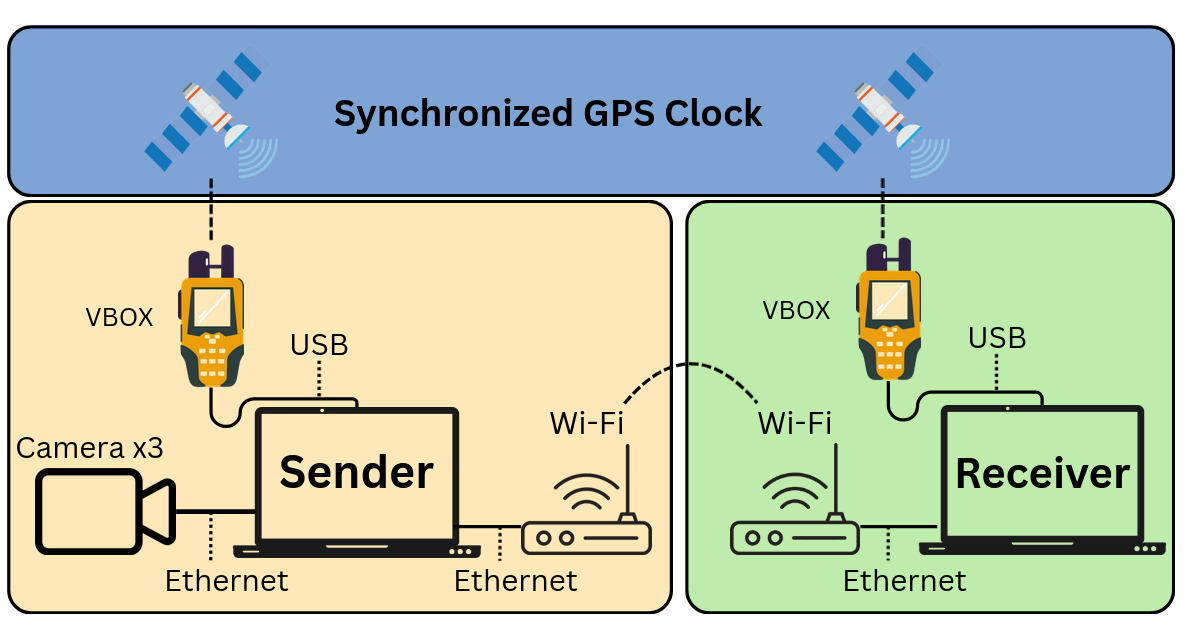
\includegraphics[width=0.9\textwidth]{Images/System/PhysicalSetup.png}
    \caption{Physical Setup of Project}\label{fig:physicalSetup}
\end{figure}

\begin{figure}[h]
    \centering
    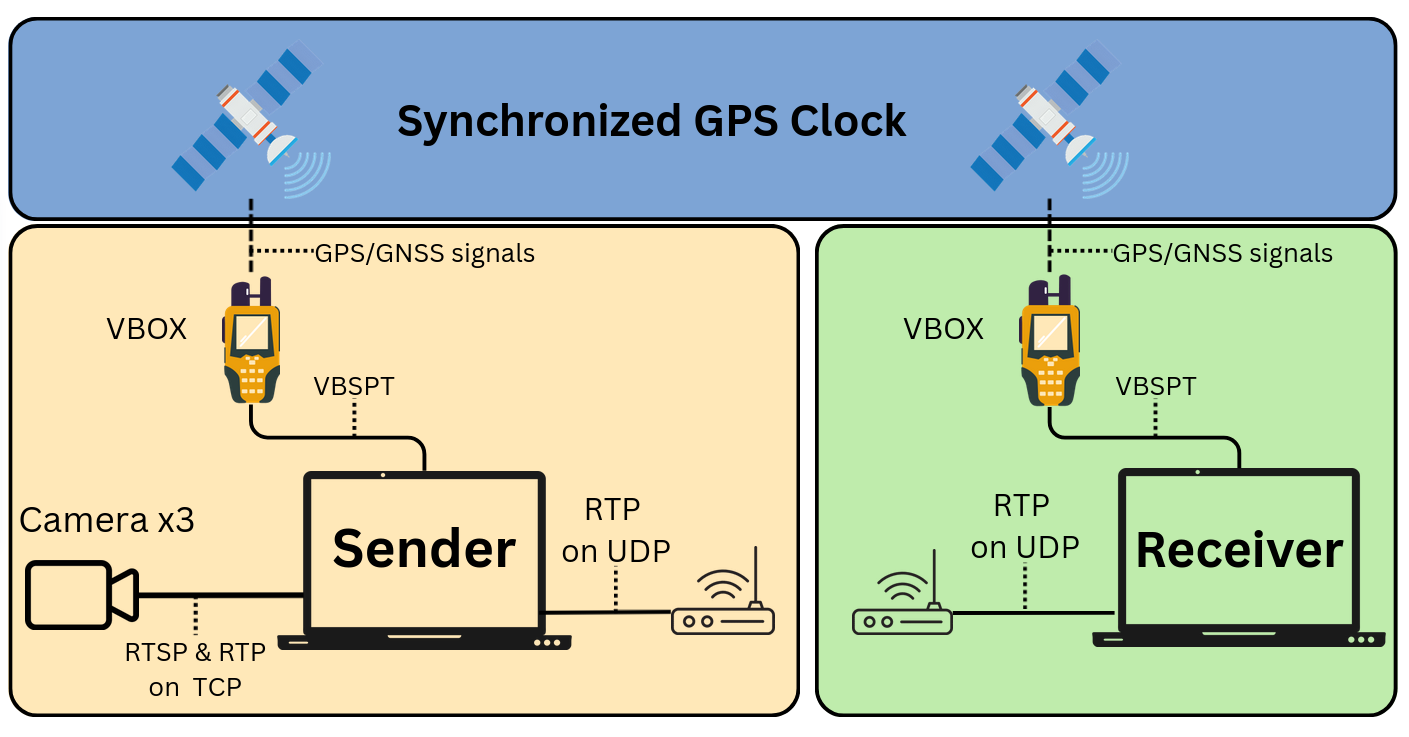
\includegraphics[width=0.9\textwidth]{Images/System/ApplicationAndTransportSetup.png}
    \caption{Application and Transport Layer Setup of Project}\label{fig:appAndTransSetup}
\end{figure}

At the application layer, the sender pulls video from each camera using RTSP over TCP, passing the videostream through a network switch into the same ethernet interface on the computer where it is transcoded or re encoded with the active configuration, packages the result into RTP, and transmits it to the receiver over UDP (or TCP for specific configurations). The receiver listens on a dedicated UDP port per camera, depay loads the RTP stream, decodes the video, and renders it to the display. Clock timestamps injected at the sender are compared against arrival timestamps on the receiver to compute end-to-end latency.

\subsection{Components}

The system is built from the following physical and software components.

\textbf{Cameras.} Three Hikvision IP cameras serve as the video sources. Each camera is assigned a static IP address using the SADP and iVMS management tools and will retain that address until manually changed. The cameras encode video internally and expose it over RTSP on TCP port 554. Before opening a stream, the sender pings each camera IP address to confirm reachability and uses NetCat to verify that the RTSP port is available.

\textbf{Network switch.} The three cameras connect to the sender through a network switch over Ethernet. This allows all cameras to share a single physical interface on the sender while remaining individually addressable by their static IP addresses.

\textbf{Sender computer.} A Linux laptop running Ubuntu acts as the sender. It connects to the camera switch over Ethernet and to the internet through a 5G modem, also over Ethernet. The GStreamer sender pipeline runs on this machine, pulling streams from all three cameras and forwarding the processed video to the receiver over the internet via Tailscale.

\textbf{5G modem.} A 5G modem provides the sender with internet connectivity. This reflects the intended deployment context of a moving train, where a cellular uplink is the realistic means of connecting to a remote operator station.

\textbf{Receiver computer.} A second Linux laptop acts as the receiver. It connects to the internet through a standard Wi-Fi router and listens on a dedicated UDP port per camera stream. A GStreamer receive pipeline on this machine decodes and displays each incoming stream.

\textbf{Network and addressing.} Tailscale is installed on both machines and configured under the same account, giving each machine a stable virtual IP address. This means the sender can always reach the receiver at a fixed address regardless of which physical network either machine is connected to, making the setup straightforward to move between locations without changing any configuration.

\textbf{Clock synchronisation.} Both machines synchronise their system clocks against public internet time servers, specifically time.cloudflare.com, time.google.com, and time.apple.com, using Chrony. This provides a shared time reference between the sender and receiver, which is required for accurate one-way latency calculation. The synchronisation approach is described in more detail in Section~\ref{sec:measurementdesign}.


\subsection{Architecture}

At the application layer, the sender opens an RTSP session with each camera over TCP and pulls the video stream across the local Ethernet network. The camera delivers video as RTP encapsulated within the TCP connection in interleaved mode, where one channel carries the RTP video data and a second channel carries RTCP for control feedback and quality monitoring. The use of TCP on this local segment is appropriate because the wired connection between the switch and the sender is short and reliable, meaning the overhead of TCP does not introduce meaningful latency while the reliability guarantee simplifies session management.

Once the sender has received the stream from a camera, it processes and re-encodes the video according to the active test configuration and packages the result into new RTP packets. These packets are then transmitted to the receiver over the internet via Tailscale using UDP. UDP is selected as the default transport for this segment because it introduces no connection overhead or retransmission delay, both of which would add directly to end-to-end latency. The behaviour of the pipeline under degraded network conditions where UDP packet loss occurs is examined explicitly in the experimental evaluation.

The receiver listens on a separate UDP port for each of the three camera streams, ports 5000, 5002, and 5004 respectively. Assigning a distinct port per stream allows all three to be received simultaneously on the same machine without any additional routing logic.

It is important to distinguish between the transport layer and the application layer in this setup. TCP and UDP operate at the transport layer and govern how packets are delivered between the two machines. RTSP and RTP operate at the application layer and govern how the video stream is described, negotiated, and carried within those packets. The sequence diagram in Figure~\ref{fig:seqDiagramRTSP} illustrates the exchange that takes place between the sender and a camera before an active video stream begins.

\begin{figure}[h]
    \centering
    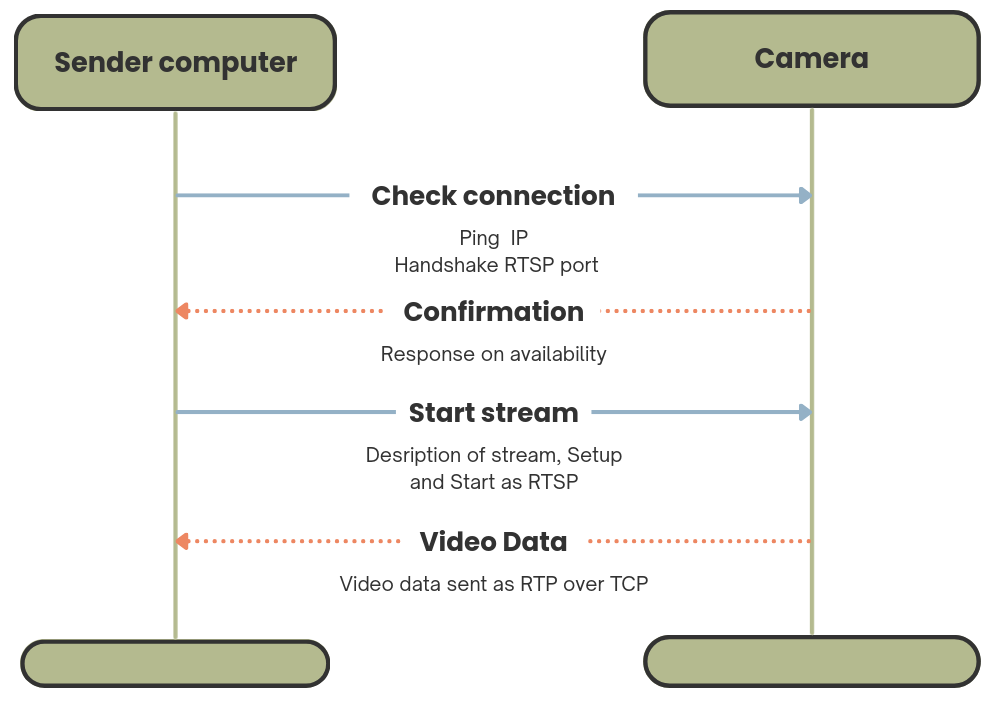
\includegraphics[width=0.9\textwidth]{Images/System/SequenceDiagramCompCam.png}
    \caption{Sequence Diagram between Sender and Camera before Active Stream}\label{fig:seqDiagramRTSP}
\end{figure}


\subsection{Pipeline Design}

GStreamer is used as the media processing framework on both machines. Each camera is handled by an independent pipeline instance on the sender, and each stream is received by an independent pipeline instance on the receiver. Running separate pipelines per camera keeps failure domains isolated, meaning a problem on one stream does not interrupt the others, and it makes adding or removing a camera as simple as starting or stopping one pipeline instance.

\subsubsection{Sender Pipeline}

The sender pipeline for each camera follows this element chain:

\begin{verbatim}
rtspsrc -> rtph264depay -> queue -> rtph264pay -> queue -> udpsink
\end{verbatim}

\textbf{rtspsrc} opens the RTSP session with the camera over TCP and pulls the incoming RTP stream. The \texttt{latency} property is set to 0, disabling the internal jitter buffer. On a wired local connection the variation in packet arrival timing is very small, so buffering would add a fixed delay without a meaningful reliability benefit.

\textbf{rtph264depay} strips the RTP packetisation to produce raw H.264 NAL units. Although the payload is re-packetised immediately downstream, this step serves two purposes. It creates a clean interception point for the latency measurement probe described in Section~\ref{sec:measurementdesign}, and it allows any intermediate processing such as transcoding or scaling to be inserted between the depay and repay elements without restructuring the rest of the pipeline. The \texttt{config-interval} property on the downstream payloader is set to \texttt{-1}, causing SPS and PPS parameter sets to be injected into every keyframe so that a receiver joining mid-stream can synchronise without delay.

\textbf{rtph264pay} re-packetises the NAL units into RTP packets ready for transmission.

\textbf{udpsink} sends the RTP packets to the receiver Tailscale address on the port assigned to that camera. For the TCP transport variant tested in the experimental evaluation, \texttt{udpsink} is replaced by \texttt{tcpclientsink} with equivalent addressing.

When transcoding is active, for example when evaluating H.265 or MJPEG, or when moving encoding from the camera hardware to the sender CPU or GPU, additional elements are inserted between \texttt{rtph264depay} and the output payloader. The exact element chains for each tested configuration are listed in Chapter~\ref{chap:methodology}.

\subsubsection{Receiver Pipeline}

The receiver pipeline for each stream follows this element chain:

\begin{verbatim}
udpsrc -> rtph264depay -> h264parse -> avdec_h264 -> queue -> autovideosink
\end{verbatim}

\textbf{udpsrc} listens on the UDP port assigned to the stream.

\textbf{rtph264depay} strips the RTP encapsulation to recover H.264 NAL units.

\textbf{h264parse} parses the bitstream and structures it into well-formed access units, handling tasks such as verifying stream parameter sets and ensuring that downstream elements receive properly delimited frame boundaries.

\textbf{avdec\_h264} performs software H.264 decoding to produce raw frames. This is the most computationally demanding step in the receiver pipeline.

\textbf{autovideosink} renders each decoded frame to the display. The \texttt{sync} property is set to \texttt{false}, which causes frames to be displayed as soon as they are decoded rather than waiting for the presentation time embedded in the stream. This removes a potential source of added latency at the cost of not enforcing frame pacing.


\subsection{Measurement Design}\label{sec:measurementdesign}

Accurate end-to-end latency measurement across two separate machines requires that both share a common time reference. As described in Section~\ref{sec:clocksync}, both machines synchronise to public internet time servers via Chrony. Under stable conditions this provides clock agreement within a few milliseconds, which is small relative to the pipeline latency values being measured and is acknowledged when interpreting results.

Timestamps are captured using GStreamer probes attached to pads at two points in the pipeline. On the sender, a probe is placed on the source pad of \texttt{rtph264pay}, recording the system time at which each RTP packet leaves the sender pipeline. On the receiver, a probe is placed on the sink pad of \texttt{autovideosink}, recording the system time at which the corresponding decoded frame arrives for display. The RTP sequence number carried in each packet is used to match sender and receiver records for the same frame.

End-to-end latency for each frame is then computed as:

\begin{equation}
  L = T_{\text{receiver}} - T_{\text{sender}}
\end{equation}

where $T_{\text{sender}}$ is the timestamp recorded at the sender probe and $T_{\text{receiver}}$ is the timestamp recorded at the receiver probe for the matching sequence number.

This measurement boundary captures encoding, packetisation, network transmission, depayloading, decoding, and the presentation queue. Camera capture latency and physical display rendering time fall outside this boundary, as they occur before and after the instrumented portion of the pipeline respectively and are considered largely constant across configurations. The practical consequence of this boundary is discussed further in Section~\ref{chap:discussion}.

Timestamps and sequence numbers are written to CSV log files on each machine during each test run. Post-processing matches sender and receiver records by sequence number, discards frames for which no receiver record exists due to packet loss, and computes per-frame latency, mean latency, and standard deviation for each configuration.


\subsection{Network Setup}

During testing, the sender and receiver communicate over the internet via Tailscale. The sender connects through a 5G modem and the receiver connects through a Wi-Fi router, reflecting a realistic asymmetric setup where one end of the link uses a cellular uplink and the other uses a fixed broadband connection.

Tailscale is installed on both machines and logged in under the same account, providing each machine with a stable virtual IP address in the 100.x.x.x range. All outgoing RTP streams from the sender are addressed to the receiver Tailscale IP, which means the same scripts and configuration files work regardless of which physical network either machine is connected to.

Firewall rules on the receiver are configured to accept inbound UDP traffic on ports 5000, 5002, and 5004 to ensure that the operating system does not silently drop incoming stream packets.

For the bandwidth-limited test conditions, a software traffic shaper is applied on the sender network interface to impose an upper bitrate ceiling, simulating a degraded or congested link. This allows the effect of reduced available bandwidth to be evaluated in a controlled and repeatable way without depending on naturally occurring network congestion.

